\chapter{Shell环境管理}
\label{cp:shellmgr}

\section{Shell中的任务控制}

\subsection{概述(前台任务与后台任务)}

我们需要首先明确,在Shell中,\textbf{进程管理包括前台任务和后台任务的控制}。\textit{每个进程都可以在前台运行,接受用户的直接输入和输出,或在后台运行,不影响用户继续在终端执行其他命令。}\\

所谓\textbf{前台任务},即\textit{Foreground Job},就是指一个进程在前台运行时,用户会等待它执行完成后才能继续输入命令。类似的,\textbf{后台任务}\textit{Background Job},就是进程在后台运行时,不会占用Shell的控制权,用户可以继续操作其他任务。\\

我们根据定义可以知晓,其实\textit{所谓前、后台,都是Shell相对于用户的一个概念},即\textit{用户是否能够直接与进程进行交互,如能,则为前台任务,否则为后台任务}。\\

有了上述的概念,我们就可以开始探讨\textbf{如何在Shell中控制任务}了。

\subsection{任务控制的基本操作}

首先我们需要明确,在Shell中\textbf{任务共有三种状态},即\textit{运行、挂起、终止}。我们通过一些常用的指令来控制任务的状态。

\begin{itemize}
    \item \texttt{Ctrl + Z}:将当前任务挂起(即将任务转为后台任务)。
    \item \texttt{Ctrl + C}:终止当前任务。
    \item \texttt{Ctrl + D}:终止当前Shell会话。
    \item \texttt{bg}:将任务转为后台任务。
    \item \texttt{fg}:将任务转为前台任务。
    \item \texttt{jobs}:查看当前Shell中的任务。
\end{itemize}

下面我们给出一些示例,在我的\texttt{Ubuntu Azure SG}服务器上进行测试,来具体化解释这些指令的用法。\\

第一组示例,我们将示范如何将单个任务转为后台任务\footnote{至于为什么强调\textit{单个},因为如果有多个进程须指定任务号。如果只有一个进程,则不需指定任务号(除非使用\texttt{kill})},见\autoref{listing:taskcontrol1}。

\begin{longlisting}
    \begin{minted}{bash}
wget -c --limit-rate=10k https://releases.ubuntu.com/noble/ubuntu-24.04.1-live-server-amd64.iso # 以 -c 允许断点续传,以 --limit-rate=10k 限速下载

# 此时任务在前台运行,我们可以按下 Ctrl + Z 将任务挂起
^D # Ctrl + Z 将任务挂起
# 将提示 [1]+  Stopped  wget -c --limit-rate=10k https://... 任务已经被挂起

bg # 将任务转为后台任务
# 此时控制台提示 [1]+ wget -c --limit-rate=10k https://... & 任务已经转为后台任务
# 并提示 Redirecting output to ‘wget-log’.

jobs # 使用 jobs 验证之
# 此时控制台提示 [1]+  Running  wget -c --limit-rate=10k https://... &

# 若要在此时直接终止进程,使用:
kill %1 # 杀死后台任务

# 或者将任务转为前台任务,再终止:
fg # 可以将任务转为前台任务
# 此时任务又转为前台任务
^C #Ctrl + C 以终止任务
    \end{minted}
    \caption{任务控制实例一:以后台任务运行}
    \label{listing:taskcontrol1}
\end{longlisting}

第二组示例,我们将示范如何同时对多个进程进行任务控制,见\autoref{listing:taskcontrol2}。

\begin{longlisting}
    \begin{minted}{bash}
sleep 1000 & # 启动一个后台任务,其中 & 表示后台运行
# 此时控制台提示 [1] 629227 任务号和PID号
sleep 2333 & # 再启动一个后台任务
# 此时控制台提示 [2] 629228 任务号和PID号
sleep 1234 & # 再启动一个后台任务
# 此时控制台提示 [3] 629229 任务号和PID号
jobs
# 控制台返回
# [1]   Running                 sleep 1000 &
# [2]-  Running                 sleep 2333 &
# [3]+  Running                 sleep 1234 &
# 特别的,任务号后的 + 表示当前任务,- 表示上一个任务,无符号表示其他任务
# 这些任务都在并行运行,通过
ps -ef | grep sleep
# JStar0   629227  629216  0 15:35 pts/1    00:00:00 sleep 1000
# JStar0   629228  629216  0 15:35 pts/1    00:00:00 sleep 2333
# JStar0   629229  629216  0 15:35 pts/1    00:00:00 sleep 1234
# 可以看到这三个任务都在后台运行

fg %2 # 将任务2转为前台任务
# 此时返回 sleep 2333 任务转为前台任务
^C # Ctrl + C 以终止任务

kill %1 %3 # 杀死任务1和任务3
# 此时返回
# [1]-  Terminated              sleep 1000
# [3]+  Terminated              sleep 1234

jobs
# 此时不返回任何任务,所有任务都已经终止
    \end{minted}
    \caption{任务控制实例二:对多个任务进行控制}
    \label{listing:taskcontrol2}
\end{longlisting}

\section{深入探索信号机制}

\subsection{信号在进程管理的概念}

类Unix系统中,信号是一种\textbf{软件中断},\textit{允许操作系统和进程之间进行通信}。信号的发送者,可以是\textit{操作系统、硬件或用户},将给\textit{接收者即进程},告知执行特定的操作或响应某个事件。Shell中的进程管理\textbf{通过信号来控制}前台和后台任务。\\

参考\cite{enwiki:1243602968},在数字计算机中,中断\textit{an interrupt (sometimes referred to as a trap)}是对处理器的请求,\textit{以中断当前正在执行的代码(在允许的情况下),以便及时处理事件。}如果请求被接受,处理器将暂停其当前活动,保存其状态,并执行称为中断处理程序\textit{(或中断服务例程,ISR)}的函数来处理事件。这种中断通常是临时的,在中断处理程序完成后允许软件恢复正常活动,尽管中断也可能表示致命错误。

\subsection{常见的信号}

\textit{信号是有限的消息,用于通知进程发生了某些事件。}\textbf{每种信号都有一个编号和名称},操作系统会根据事件类型发送相应的信号给进程。常见的信号如下:

\begin{longtable}{|c|p{11cm}|}
    \hline
    \textbf{信号} & \textbf{描述} \\
    \hline
    SIGINT (信号 2) & 中断信号。当用户按下 Ctrl + C 时,系统向前台进程发送这个信号,通常用于停止进程。 \\
    \hline
    SIGKILL (信号 9) & 强制终止信号。无论进程是否忽略信号,SIGKILL 都会立即终止进程。不能被捕捉或忽略。 \\
    \hline
    SIGTERM (信号 15) & 终止信号,表示请求进程优雅地退出。进程可以捕捉这个信号并在退出前执行清理操作。 \\
    \hline
    SIGHUP (信号 1) & 挂起信号,当终端关闭时,系统会发送这个信号,通常用于告诉守护进程重新读取配置文件。 \\
    \hline
    SIGSTOP (信号 19) & 停止进程。不能被捕捉或忽略,和 SIGKILL 类似,但不会终止进程,只是暂停。 \\
    \hline
    SIGCONT (信号 18) & 继续信号,用于恢复被暂停的进程。 \\
    \hline
\end{longtable}

一般我们通过相关的命令和快捷键来发送信号,如\texttt{kill}命令,将发送信号 \texttt{SIGTERM} 给指定的进程。具体的实现细节,在使用命令和快捷键时,我们不需要关心,只需要知道\textbf{信号是一种进程间通信的方式}即可。\\

类似的,我们也可以\textbf{给出其他的对应关系}。如\texttt{Ctrl + C -> SIGINT},终止前台任务;\texttt{Ctrl + Z -> SIGTSTP},将前台任务挂起(转为后台停止状态);\texttt{bg 发送 SIGCONT},恢复挂起的任务在后台运行等。\\

使用Python中内置的\texttt{signal}库,我们也可以\textbf{捕捉信号},如\autoref{listing:signal}所示。

\begin{longlisting}
    \begin{minted}{python}
import signal, time

def signalHandler(signum, time):
    print("\n获取到信号:", signum)

signal.signal(signal.SIGINT, signalHandler)
i = 0
while True:
    time.sleep(.1)
    print("\r{}".format(i), end="")
    i += 1
    \end{minted}
    \caption{Python模拟的信号捕捉}
    \label{listing:signal}
\end{longlisting}

那么,此程序在运行时,不会因为按下\texttt{Ctrl + C}而终止,而是会输出\texttt{获取到信号: 2},即捕捉到了\texttt{SIGINT}信号。\\

这个程序的运行结果如\autoref{fig:signal}所示。

\begin{figure}[!h]
    \centering
    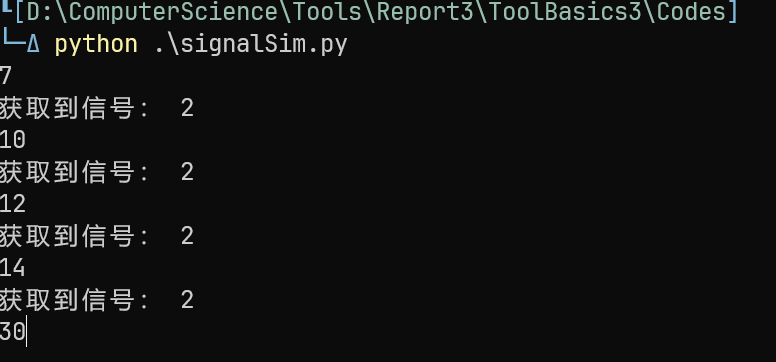
\includegraphics[width=.8\textwidth]{./Figures/signal.png}
    \caption{Python模拟的信号捕捉}
    \label{fig:signal}
\end{figure}

\section{Shell中的终端多路复用}

我们主要比较两种常见的终端多路复用工具,即\texttt{screen}和\texttt{tmux}。

\subsection{功能比较}

我们给出一个简单的功能比较表,见\autoref{tab:tmuxvsscreen}所示。

\begin{longtable}{|p{2cm}|p{6cm}|p{6cm}|}
    \hline
    \textbf{功能/特性} & \textbf{tmux} & \textbf{screen} \\
    \hline
    \endfirsthead

    \hline
    \textbf{功能/特性} & \textbf{tmux} & \textbf{screen} \\
    \hline
    \endhead
    
    \hline
    \endfoot
    
    \hline
    \endlastfoot
    
    会话管理 & 可以命名、分离、重新连接和恢复多个会话 & 同样支持会话的分离和恢复 \\
    \hline
    窗口布局 & 提供灵活的窗口布局,可以分屏(水平/垂直) & 支持分屏,但功能较基础 \\
    \hline
    滚动缓冲区 & 默认支持滚动缓冲区,使用快捷键轻松滚动 & 需要手动启用滚动缓冲区,操作较繁琐 \\
    \hline
    配置文件 & 配置文件位于 ~/.tmux.conf,支持更复杂的配置 & 配置文件位于 ~/.screenrc,配置功能较少 \\
    \hline
    会话共享 & 支持会话共享,允许多个用户连接同一个会话 & 同样支持会话共享 \\
    \hline
    插件扩展 & 支持插件扩展,可以通过 tmux 插件管理器安装扩展 & 不支持插件扩展 \\
    \hline
    状态栏 & 可高度自定义状态栏 & 状态栏不可定制 \\
    \hline
    复制模式 & 内置复制模式,使用更简单 & 支持复制模式,但需要额外配置 \\
    \hline
    热键风格 & 默认热键风格现代,易于使用 & 热键风格传统,学习成本稍高 \\
    \hline

    \caption{tmux与screen功能比较}
    \label{tab:tmuxvsscreen}
    
\end{longtable}

\subsection{指令上的比较}

基于我对\texttt{screen}的认识和对\texttt{tmux}的学习,给出一个简单的指令比较表,如\autoref{tab:tmuxvsscreencmd}所示。

\begin{longtable}{|l|l|l|}
    \hline
    \textbf{功能/操作} & \textbf{tmux 指令} & \textbf{screen 指令} \\
    \hline
    \endfirsthead

    \hline
    \textbf{功能/操作} & \textbf{tmux 指令} & \textbf{screen 指令} \\
    \hline
    \endhead

    \hline
    \endfoot

    \hline
    \endlastfoot

    启动新会话 & tmux new -s <session\_name> & screen -S <session\_name> \\
    \hline
    分离会话 & Ctrl + b 然后按 d & Ctrl + a 然后按 d \\
    \hline
    重新连接会话 & tmux attach -t <session\_name> & screen -r <session\_name> \\
    \hline
    列出所有会话 & tmux ls & screen -ls \\
    \hline
    关闭会话 & tmux kill-session -t <session\_name> & screen -S <session\_name> -X quit \\
    \hline
    创建新窗口 & Ctrl + b 然后按 c & Ctrl + a 然后按 c \\
    \hline
    在窗口间切换 & Ctrl + b 然后按 数字键 (0-9) & Ctrl + a 然后按 数字键 (0-9) \\
    \hline
    关闭当前窗口 & exit 或 Ctrl + b 然后按 \& & exit 或 Ctrl + a 然后按 K \\
    \hline
    水平分屏 & Ctrl + b 然后按 \% & Ctrl + a 然后按 ` \\
    \hline
    垂直分屏 & Ctrl + b 然后按 " & Ctrl + a 然后按 S \\
    \hline
    在面板间切换 & Ctrl + b 然后按 箭头键 & Ctrl + a 然后按 Tab \\
    \hline
    调整面板大小 & Ctrl + b 然后按 : 输入 resize-pane & Ctrl + a 然后按 Ctrl + 箭头键 \\
    \hline
    重命名窗口 & Ctrl + b 然后按 , & Ctrl + a 然后按 A \\
    \hline
    重命名会话 & tmux rename-session -t <old\_name> <new\_name> & 不支持 \\
    \hline
    会话共享 & tmux attach -t <session\_name> & screen -x <session\_name> \\
    \hline

    \caption{tmux与screen指令比较}
    \label{tab:tmuxvsscreencmd}

\end{longtable}

\subsection{实机测试}

在实机上对我新学习的\texttt{tmux}进行了简单的测试,如\autoref{listing:testtmux}所示。

\begin{longlisting}
    \begin{minted}{bash}
tmux new -s test # 创建一个名为 test 的会话
# 此时会话已经创建,可以在其中执行命令

# 假设执行了一些命令,现在需要分离会话
# Ctrl + b 然后按 d 分离会话

tmux ls # 列出所有会话
# 此时会列出所有会话,包括 test

tmux attach -t test # 重新连接 test 会话
# 此时会重新连接到 test 会话

# 假设执行了一些命令,现在需要关闭会话

exit # 退出会话
# 此时会话已经关闭

tmux ls # 再次列出所有会话
# 此时会列出所有会话,不再包括 test
    \end{minted}
    \caption{tmux实机测试}
    \label{listing:testtmux}
\end{longlisting}


\section{远程设备的操作}

\textbf{使用SSH连接到远程设备,是我们用来控制服务器、远程调试开发设备等的重要手段。}\textit{SSH就是Secure Shell Protocol},是一种加密的网络协议,即使在不安全的网络上也能够安全地运行网络服务。\\

下面给出一个简单的SSH连接示例,是我通过OpenSSH连接到我的Azure SG服务器的过程,如图\autoref{fig:ssh1}所示。

\begin{figure}[!h]
    \centering
    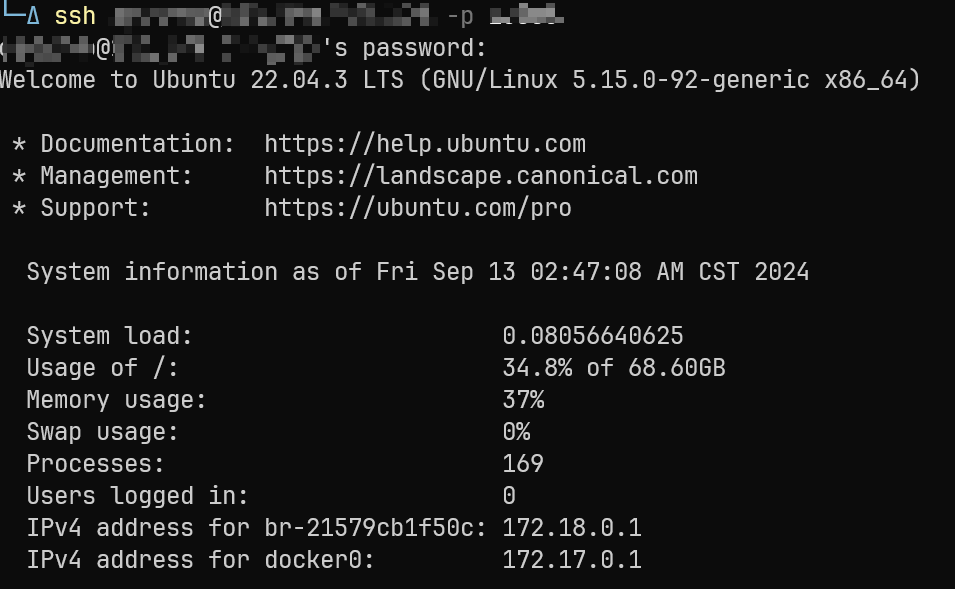
\includegraphics[width=.8\textwidth]{./Figures/ssh1.png}
    \caption{终端的SSH示例}
    \label{fig:ssh1}
\end{figure}

当然,我们还可以使用更先进的带GUI的SSH客户端,如我常用的\texttt{termius},如图\autoref{fig:ssh2}所示。

\begin{figure}[!h]
    \centering
    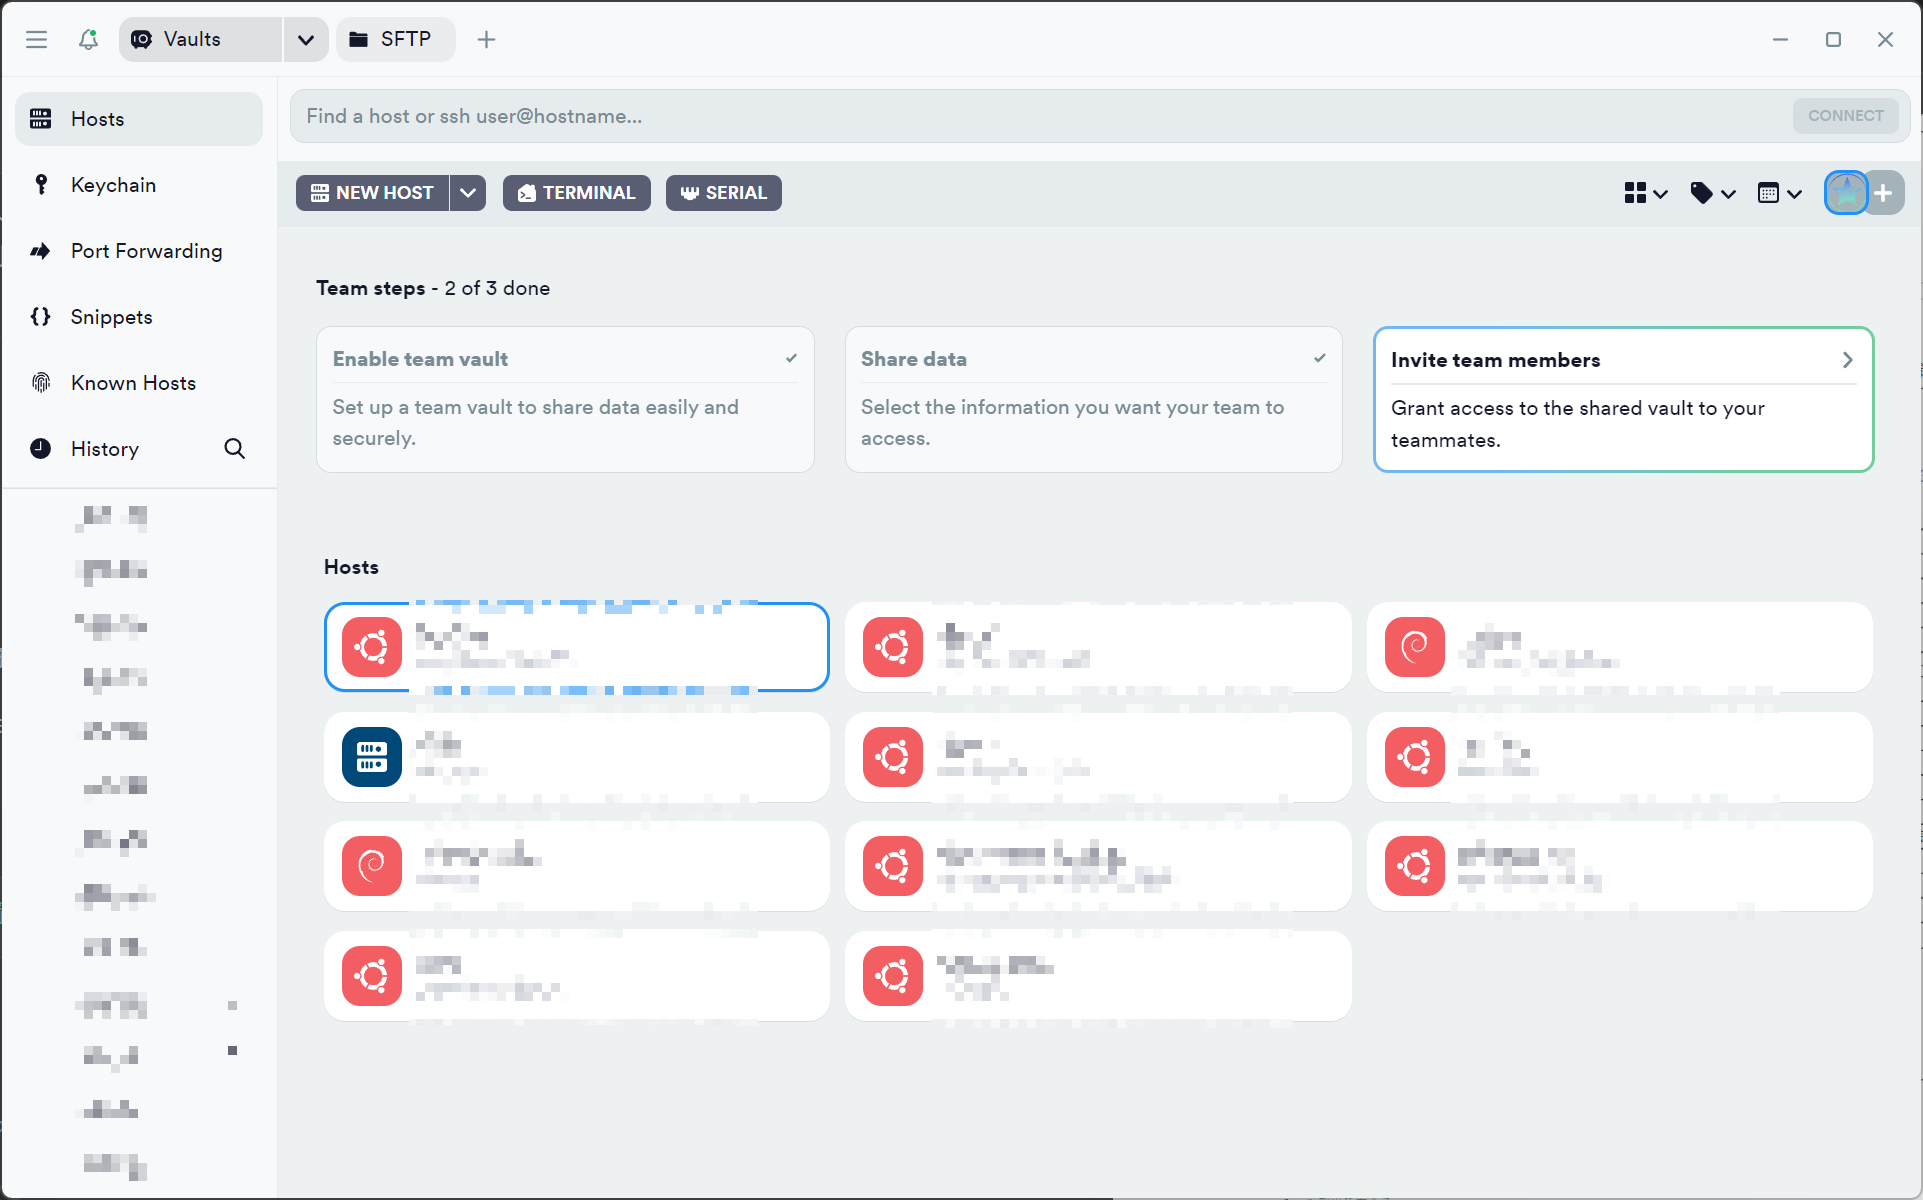
\includegraphics[width=.8\textwidth]{./Figures/ssh2.png}
    \caption{使用Termius连接示例}
    \label{fig:ssh2}
\end{figure}

\section{小结}

本章,我们首先\textbf{介绍了Shell中的任务控制},\textit{包括前台任务和后台任务的概念,以及如何通过一些常用的指令来控制任务的状态}。然后我们\textbf{深入探讨了信号机制},\textit{介绍了信号的概念和常见的信号}。最后我们\textbf{比较了两种常见的终端多路复用工具}\texttt{tmux}和\texttt{screen},并\textit{给出了功能比较和指令比较}。最后我们简单介绍了\textbf{远程设备的操作},即\textit{通过SSH连接到远程设备}。